% set counter to n-1:
%\setcounter{chapter}{1}

\chapter{Related Work}
\label{chap:related}
A lot of software for the purpose of 3D modelin exists, with some of the best known ones being Maya, Blender, Autodesk 3ds Max and Zbrush~\cite{Maya, Blender, 3dsMAX, ZBrush}. Typically these software let their users manipulate meshes on vertex, edge or face level, resulting in very fine-grained control over the appearance of created models. Although this makes these programs very powerful and versatile for the creation and editing 3D models, they come with a very steep learning curve and are overcomplete for recreational users. This chapter instead focusses on describing some of the more intuitive and easy-to-use sketch-based 3D modeling software, as well as a couple of relatively new software for creating 3D content in VR. 

\section{Sketch-based Modeling}
Sketch-based modeling is a modeling technique that aims to transfer the way that people draw shapes with pen and paper to a method of modeling 3D shapes on the PC with a mouse. With the mouse the user draws strokes on the screen, whose interior is subsequently meshed and then inflated to smooth rotund 3D meshes. Typically the user can then edit this initial mesh by specifying additional strokes that for example create extrusions or cut the mesh.
The software that was written as part of this thesis also adopts the sketch-based modeling paradigm. 


\subsection{FiberMesh}
\label{subsec:fiber}
FiberMesh is a system that allows modeling freeform surfaces by drawing and editing 3D curves~\cite{Nealen2007}. The user-defined curves are used to create a 3D model and stay present on the model and can be used to edit the geometry. This allows for a very intuitive method of deforming and editing meshes after their initial creation. FiberMesh lets users define curves as smooth or sharp, add and remove control curves on the mesh and pull curves to deform the mesh. Additionally it allows the user to change the mesh topology by cutting parts of the mesh and creating extrusions or tunnels.

Algorithmically FiberMesh depends on two main steps, namely curve deformation and surface optimization. In addition to these two steps, there are also a mesh construction and remeshing step, which only occur after new mesh topology has been created (e.g.\ after creation, cut or extrusion). 

For curve deformation they used a detail-preserving deformation method that combines differential coordinates~\cite{Sorkine2006} with co-rotational methods~\cite{Felippa2007}. A sequence of linear least-squares problems is solved, while satisfying the user-defined positional constraints on the drawn curves. The rotation matrices are explicitly represented as free variables, as they cannot be derived from the curves which are nearly collinear. In order to accommodate for large linear  rotations, the gross rotation is computed by iteratively concatenating small delta rotations that are each obtained by solving a linear system. The linear system that is solved in each step can be seen in equation \ref{eq:1}.  

\begin{equation} \label{eq:1}
	\arg\min_{\mathbf{v, r}} \left\lbrace \sum_{i} \left\Vert \mathbf{L}\left(\mathbf{v}_{i}\right) - \mathbf{r}_{i}\mathbf{R}_{i}\mathbf{\delta}_{i}\right\Vert^{2} + \sum_{i \in C_{1}} \left\Vert \mathbf{v}_{i} - \mathbf{v}_{i}^{'} \right\Vert^{2} + \sum_{i,j \in E}	 \left\Vert \mathbf{r}_{i}\mathbf{R}_{i} - \mathbf{r}_{j}\mathbf{R}_{j} \right\Vert^{2}_{F} + \sum_{i \in C_{2}} \left\Vert \mathbf{r}_{i}\mathbf{R}_{i} - \mathbf{R}_{i}^{'} \right\Vert^{2}_{F} \right\rbrace 
\end{equation}

Here $\mathbf{L}(\cdot)$ is the differential operator, $\mathbf{v}_{i}$ is the coordinates of vertex i, $\Vert \cdot \Vert_{F}$ is the Frobenius norm, $E$ is the set of curve edges and $C_{1}$ and $C_{2}$ are the sets of constrained vertices, primed values are constraints, $\mathbf{R}_{i}$ represents the gross rotation (in the deformed curve) corresponding to vertex i obtained from the previous iteration, and finally $\mathbf{r}_{i}$ is a linearized incremental rotation for vertex i given by a skew symmetric matrix with 3 unknowns,

\begin{equation*}
\mathbf{r}_{i} = \left[ \begin{matrix}
1 & -r_{iz} & r_{iy} \\
r_{iz} & 1 & -r_{ix} \\ 
-r_{iy} & r_{ix} & 1
\end{matrix} \right].
\end{equation*}

Rotations are updated by setting them to $\mathbf{R}_{i} = \mathbf{r}_{i}\mathbf{R}_{i}$ and orthonormalizing the result using polar decomposition~\cite{Fu2007}.
In the iterative process of estimating rotations, they use first order differentials ($L_0$), and for computing the final vertex positions using this estimated rotations they use the second order differential ($L_1$). 

\begin{equation*}
L_{0} = \mathbf{v}_{i} - \mathbf{v}_{i-1}, \quad L_{1} = \mathbf{v}_{i} - \frac{1}{\lvert N_{i} \rvert} \sum_{j \in N_{i}} \mathbf{v}_j.
\end{equation*}

For surface optimization, FiberMesh solves 3 sparse linear systems in order to compute a smooth mesh surface that adheres to the user-defined constraint curves. The first system solves for a set of smoothly varying Laplacian magnitudes $\{c_{i}\}$ which approximate the scalar mean curvature values. The least-squares minimization that it solves is as follows: 

\begin{equation}
\arg\min_{c} \left\lbrace \sum_{i} \left\Vert \mathbf{L}\left(c_{i}\right) \right\Vert^{2} + \sum_{i} \left\Vert c_{i} - c_{i}^{'} \right\Vert^{2} \right\rbrace
\end{equation}

Where $\mathbf{L\left(\cdot\right)}$ denotes the discrete graph Laplacian, which is independent of the exact mesh geometry, allowing us to reuse it in multiple iterations.
In the first iteration, the target Laplacian magnitudes are only set for the constrained curves by using the scalar mean curvature along the curve. 

To obtain a geometry that satisfies these target Laplacian magnitudes, Nealen et al.\ use the uniform Laplacian as an estimator of the integrated mean curvature normal, which is computed by $\delta_{i} = A_{i} \cdot c_{i} \cdot \mathbf{n}_{i}$, where $A_{i}$ is an area estimate for vertex i, $c_{i}$ is the target Laplacian magnitude and $\mathbf{n}_{i}$ is the estimated normal from the current face normals. However the uniform Laplacian is not an accurate estimator of the integrated mean curvature normal when the incident edges to a vertex are not of equal length. To solve for this problem without using a geometry dependent discretization and thus avoiding recomputing the matrix for every iteration, they prescribe target edge vectors in an attempt to achieve equal edge length. This is done by solving the following linear system (which uses the same matrix as the system that solves for target Laplacian magnitudes) to obtain a smooth set of target average edge lengths $e_{i}$: 

\begin{equation}
\arg\min_{e} \left\lbrace \sum_{i} \left\Vert \mathbf{L}\left(e_{i}\right) \right\Vert^{2} + \sum_{i} \left\Vert e_{i} - e_{i}^{'} \right\Vert^{2} \right\rbrace
\end{equation}

Again the first iteration is performed with only the edge lengths along the constrained curve. 
The target average edge lengths are then used to compute target edge vectors for a subset $B$ of mesh edges (in the first iteration this subset only contains edges along the constrained curves, and afterwards it contains all edges incident to the constrained curves) as follows:
\begin{equation}
\eta_{ij} = \left( e_{i} + e_{j} \right) / 2 \cdot \left( \mathbf{v}_{i} - \mathbf{v}_{j} \right) / \left\Vert \mathbf{v}_{i} - \mathbf{v}_{j} \right\Vert.
\end{equation}

These target edge vectors are then used to solve a linear system that gives the updated vertex positions as follows: 

\begin{equation}
\arg\min_{\mathbf{v}} \left\lbrace \sum_{i} \left\Vert \mathbf{L}\left(\mathbf{v}_{i}\right) - \delta_{i} \right\Vert^{2} + \sum_{i \in C} \left\Vert \mathbf{v}_{i} - \mathbf{v}_{i}^{'} \right\Vert^{2} + \sum_{\left(i,j\right) \in B} \left \Vert \mathbf{v}_{i} - \mathbf{v}_{j} - \eta_{ij} \right\Vert^{2} \right\rbrace
\end{equation}

The systems for solving for target Laplacian magnitudes, average edge lengths and optimal vertex positions are solved iteratively until convergence (approximately 5-10 iterations). Since only a geometry independent discretization of the Laplacian is used, the system matrix can be reused between iterations, until the mesh topology is changed (for example by a cutting action). Because of this, the slow matrix factorization only needs to happen once for a given mesh topology, resulting in a fast algorithm that allows for interactive rates.	

\section{3D Modeling in Virtual Reality}
\label{sec:3dmodeling}
Over the last couple of years, plenty of VR applications have been published that involve creating some type of digital 3D content. The software can roughly be split into 2 categories, namely for creating 3D paintings and for creating 3D models (assembled from a structure of vertices, edges and faces). Whereas the former category focusses on the artistic side of 3D content and usually does not result in work that can be exported to some standard format, the latter category more aims to provide a tool for producing 3D models that can be exported and then used in some other VR or 3D application. 
This section describes a variety of these 3D virtual reality applications, their interfaces and what kind of content users can make with them. 

\subsection{Google Tilt Brush}
Google's Tilt Brush is available for the Oculus Rift and HTC Vive and allows the user to  create room-scale art in the style of 3D paintings. The software provides different types of tools and brushes, including special effects tools like a fire or stars brush. Users cannot export their creations to typical model formats such as .obj or .off, but they can turn them into a GIF or upload them to Google Poly where other users can explore and enjoy their work.
Figure~\ref{fig:tiltart}~(a) shows a screenshot of example 3D artwork that has been made with Google Tilt Brush (the original work has stars that change their light intensity and seem to twinkle). In order to give the user easy access to the large set of different painting tools, Tilt Brush has created an embedded menu in the form of a painters palette that is attached to the controller in the user's non-dominant hand. Several of the menus allow for browsing through further submenus. The dominant hand is used to select a tool from the menu and paint with it. Figures~\ref{fig:tiltart}~(b) and~\ref{fig:tiltart}~(c) show two examples of what the hand-held palette menus looks like and you can see that the user can twist his hand in order to view more menu options on the backside of the palette.

\begin{figure}[t!]
    \centering
    \setlength{\tabcolsep}{0.0130\linewidth}
    \begin{tabular}{@{}c@{}}
    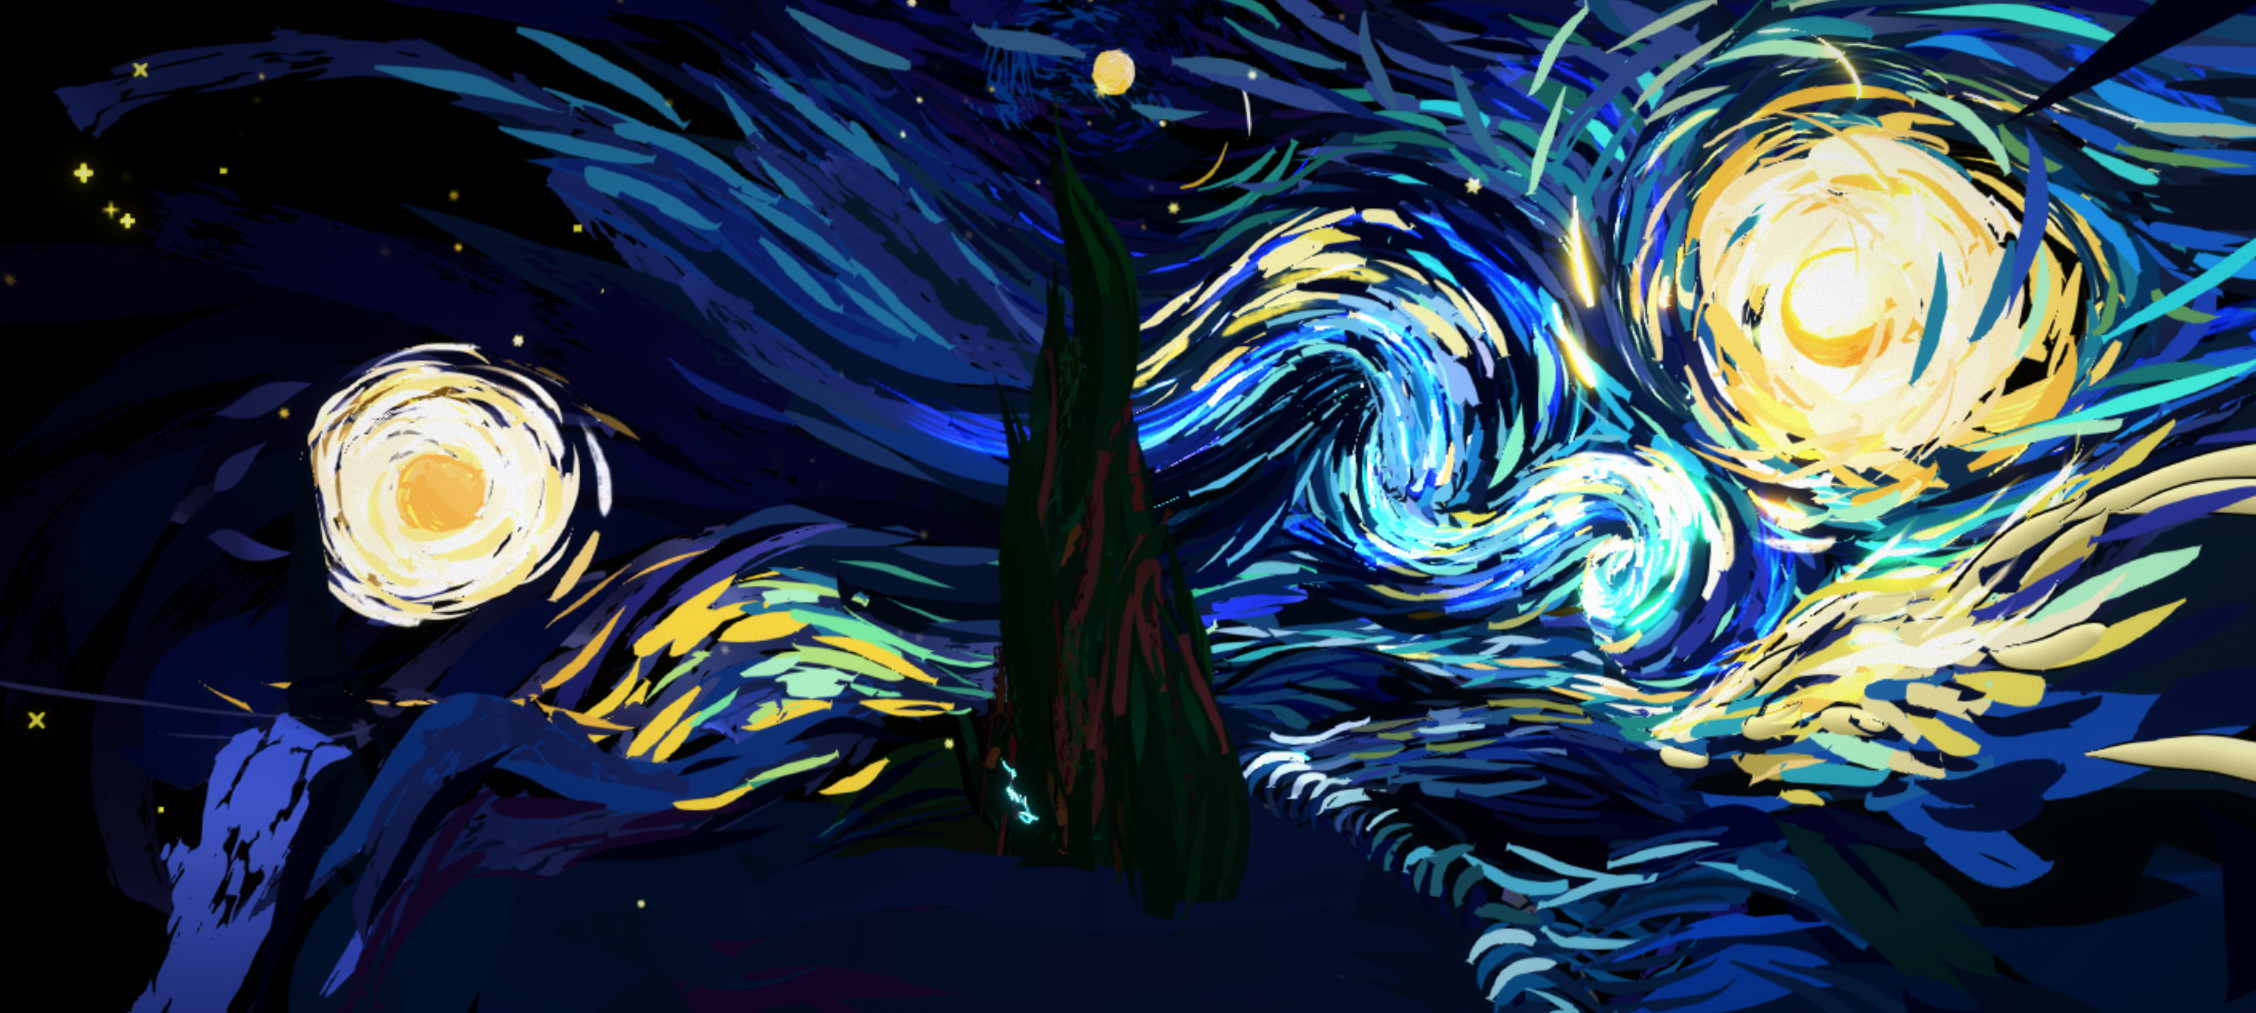
\includegraphics[width=0.7260\linewidth]{figures/TiltBrush_StarryNight}\\
    (a)
    \end{tabular}
    
    \centering
    \setlength{\tabcolsep}{0.0130\linewidth}
    \begin{tabular}{@{}cc@{}}
   	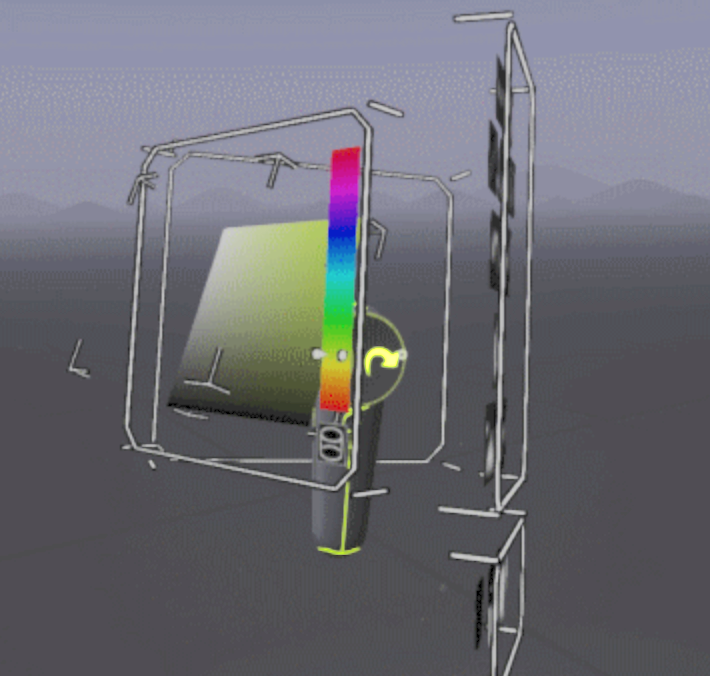
\includegraphics[width=0.35\linewidth]{figures/Tilt_menu2}&
    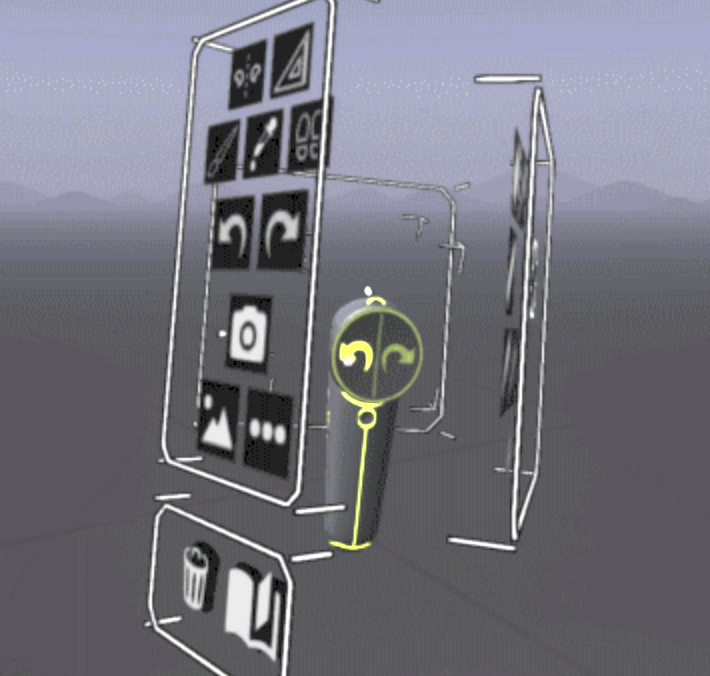
\includegraphics[width=0.35\linewidth]{figures/Tilt_menu1}\\
    (b)&(c)\\
    \end{tabular}
    \caption[Google Tilt Brush]{Google Tilt Brush.
    	  \textup{(a)} Recreation of Van Gogh's Starry Night (moving version available at https://poly.google.com/view/e-Zqenw7Dui).
			  \textup{(b)} Left-side view of the "hand-held" user interface of Google Tilt Brush. \textup{(c)} Right-side view of the "hand-held" user interface of Google Tilt Brush.
      \label{fig:tiltart}}
\end{figure}

\subsection{Oculus Medium}
Oculus Medium is a 3D sculpting tool that is only available for the Oculus Rift. Conceptually the user can paint with volumetric brushes, much like sculpting with clay. For instance the user will draw a simple circle and this will result in a donut shape. With several tools the user can sculpt away or add extra clay, as well as assigning multiple colors to the surface.
Unlike Google Tilt Brush, Oculus Medium does allow the user to store created models in .obj format, so they can be exported for use in other programs. The interface is quite intuitive since it shows a very strong connection to the method of creating 3D shapes with the use of clay in real life which most users have experience with. Users can quickly create rough shapes and refine them by adapting the brush size and adding small-scale details. The dominant hand of the user serves as the so-called "Tool hand" which can be used to sculpt with, while the non-dominant hand serves as the "Support hand" which can be used to open up several hand-held menus. Figures~\ref{fig:medium}~(a) and~\ref{fig:medium}~(b) show examples of complicated 3D models that have been made in Oculus Medium. One of the unique features of Oculus Medium is the functionality to create and use stamps, which helps easily create interesting textures on the models like the fur and grass in Figure~\ref{fig:medium}~(a).


\begin{figure}[!h]
    \centering
    \setlength{\tabcolsep}{0.0130\linewidth}
    \begin{tabular}{@{}cc@{}}
    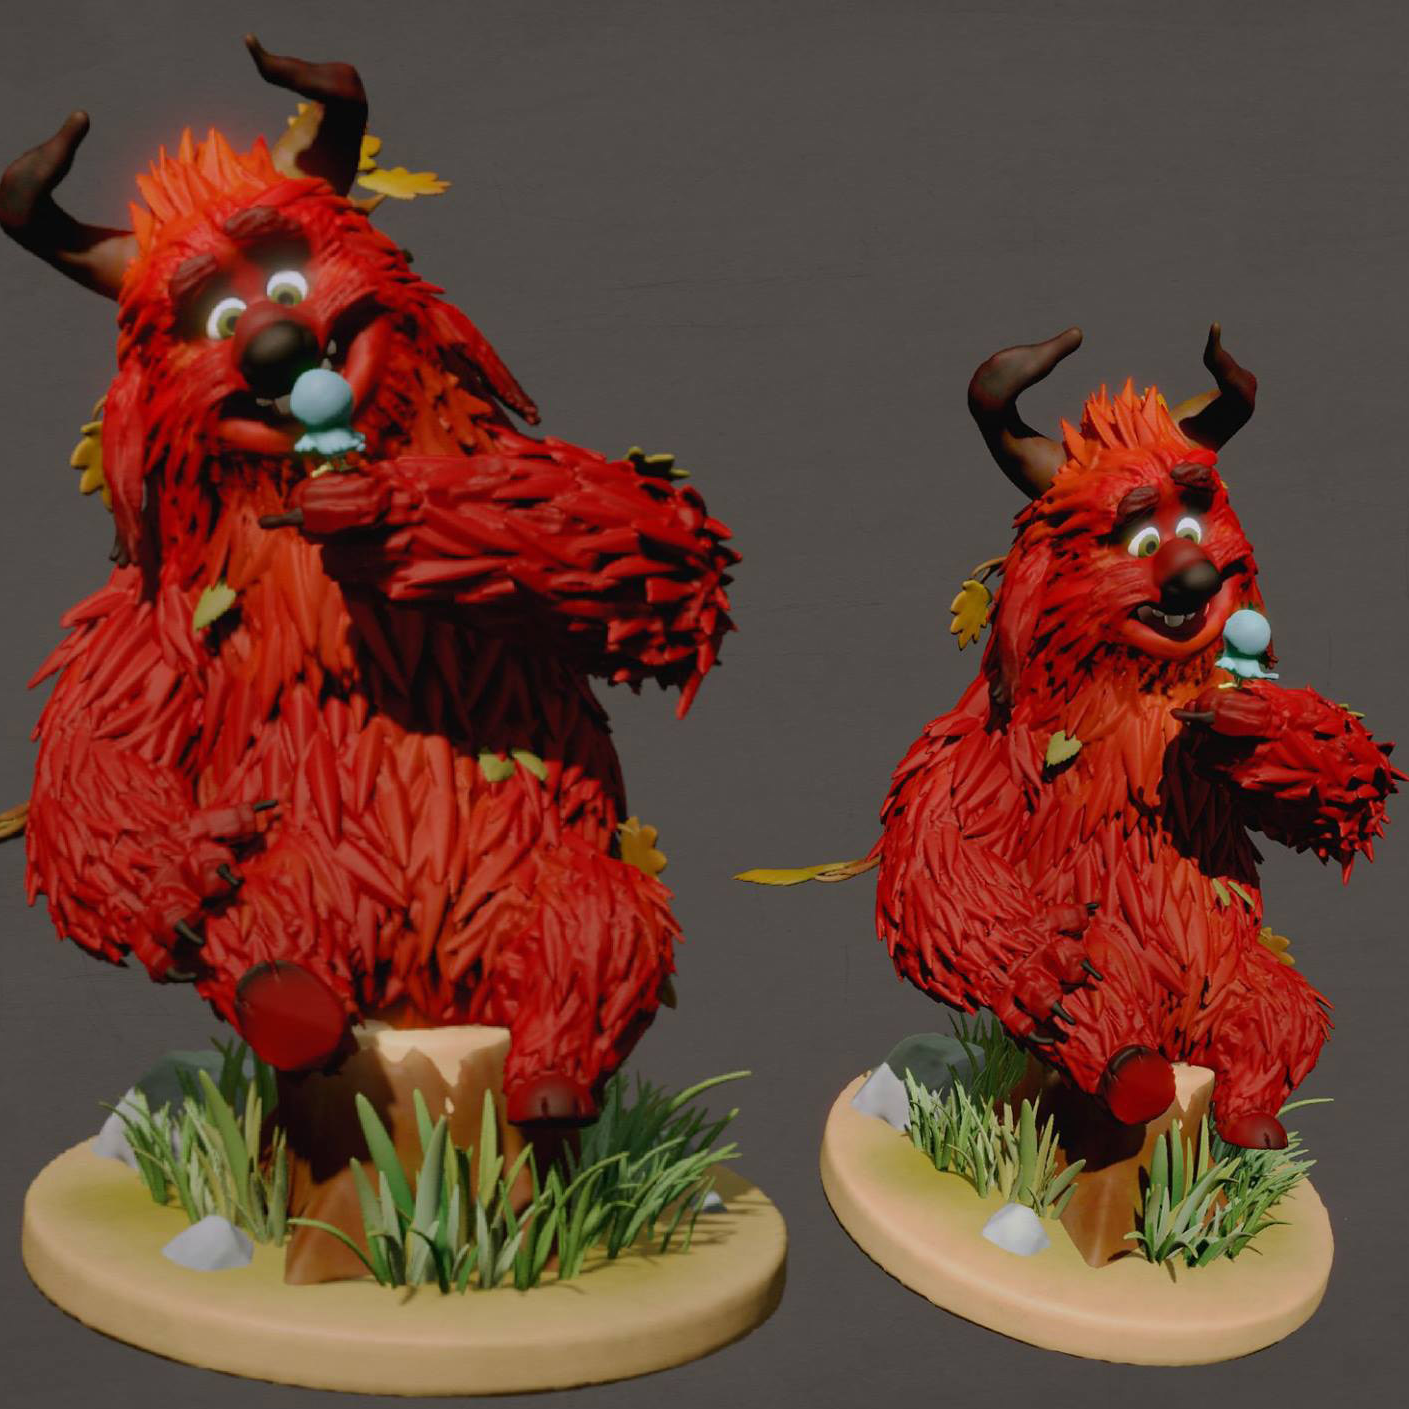
\includegraphics[width=0.35\linewidth]{figures/medium_goro_fujita} &
    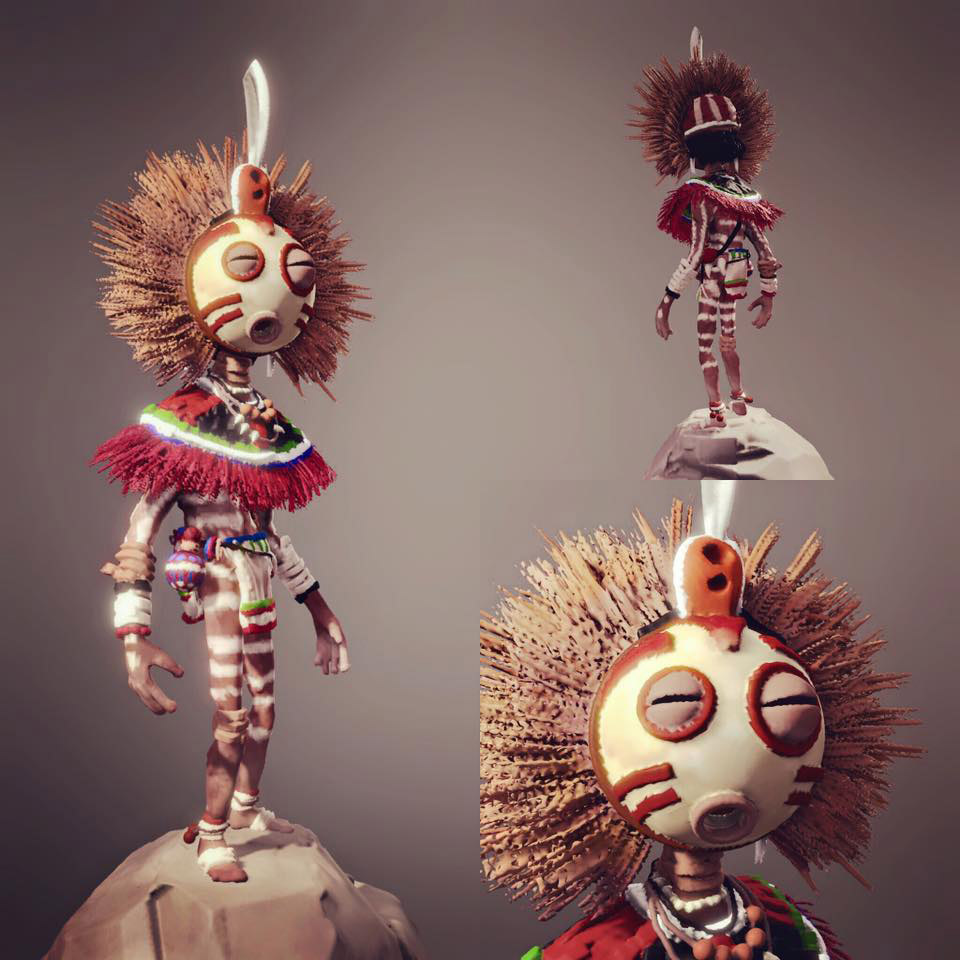
\includegraphics[width=0.35\linewidth]{figures/medium_goro_fujita2}\\

    (a)&(b)\\
    \end{tabular}
    
    \centering
    \setlength{\tabcolsep}{0.0130\linewidth}
    \begin{tabular}{@{}cc@{}}
   	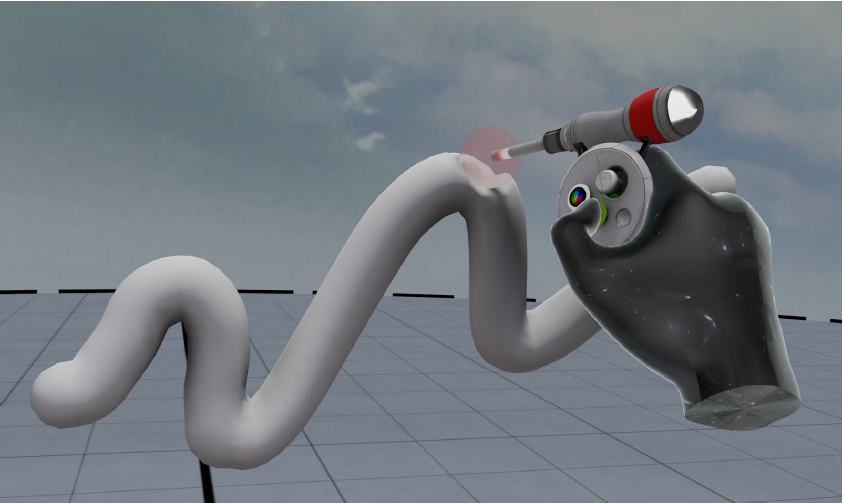
\includegraphics[width=0.35\linewidth]{figures/medium_interface1}&
   	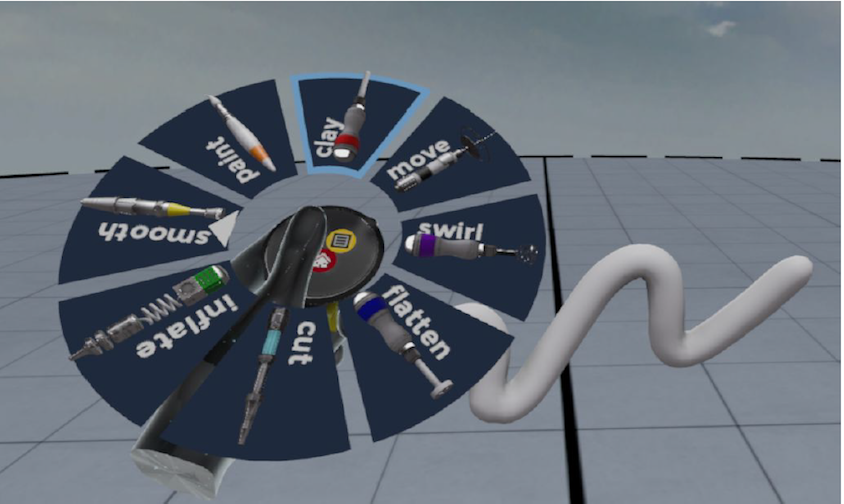
\includegraphics[width=0.35\linewidth]{figures/medium_interface2}\\
    (c)&(d)\\
    \end{tabular}
    \caption[Oculus Medium]{Oculus Medium.
    	  \textup{(a)} Model of a furry monster created in Oculus Medium by artist Goro Fujita.
			  \textup{(b)} Model of an African figure created in Oculus Medium by artist Goro Fujita. \textup{(c)} Sculpting view in Oculus Medium. \textup{(d)} Menu view in Oculus Medium.
      \label{fig:medium}}
\end{figure}

\subsection{MasterpieceVR}
MasterpieceVR brings a combination of the design paradigms used by Oculus Medium and Google Tilt Brush, letting the user mix volume sculpting with 3D painting. It is available for Oculus Rift, HTC Vive and Windows Mixed Reality, and for each of them it requires the accompanying controllers for input. One of MasterpieceVR's biggest selling points is that it allows multiple users to work on one model simultaneously, allowing interactive collaboration with direct feedback between artists. Like Oculus Medium, MasterpieceVR lets the user export models (including vertex colors) to .obj, as well as .fbx format. Additionally, users can load reference images or models into the program, which can greatly simplify modeling. MasterpieceVR implements menus in a similar fashion to Google Tilt Brush and Oculus Medium, with a menu of icons held in the user's non-dominant hand. Compared to these two, MasterpieceVR however has a larger and less intuitive menu layout. Figure~\ref{fig:masterpieceVR}~(a) shows a complex model created in MasterpieceVR and Figure~\ref{fig:masterpieceVR}~(b) shows the menu interface.

\begin{figure}[!h]
    \centering
    \setlength{\tabcolsep}{0.0130\linewidth}
    \begin{tabular}{@{}cc@{}}
   	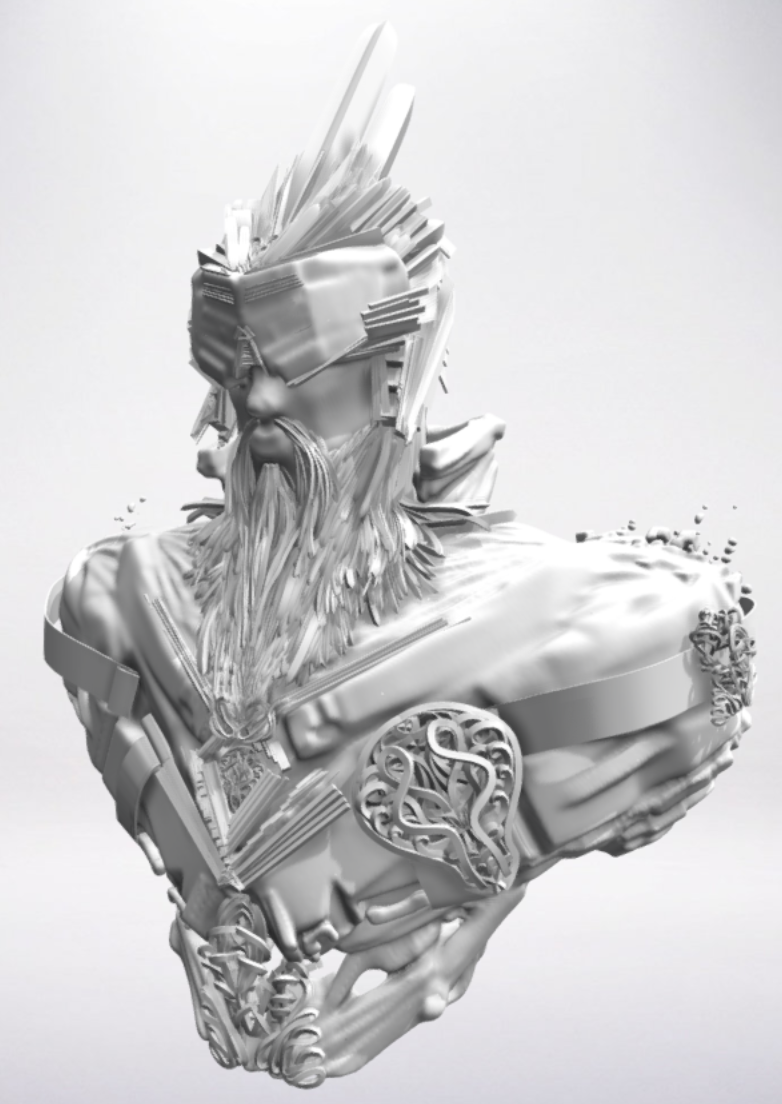
\includegraphics[width=0.35\linewidth]{figures/MasterpieceVR_Vladimir_Ilic}&
   	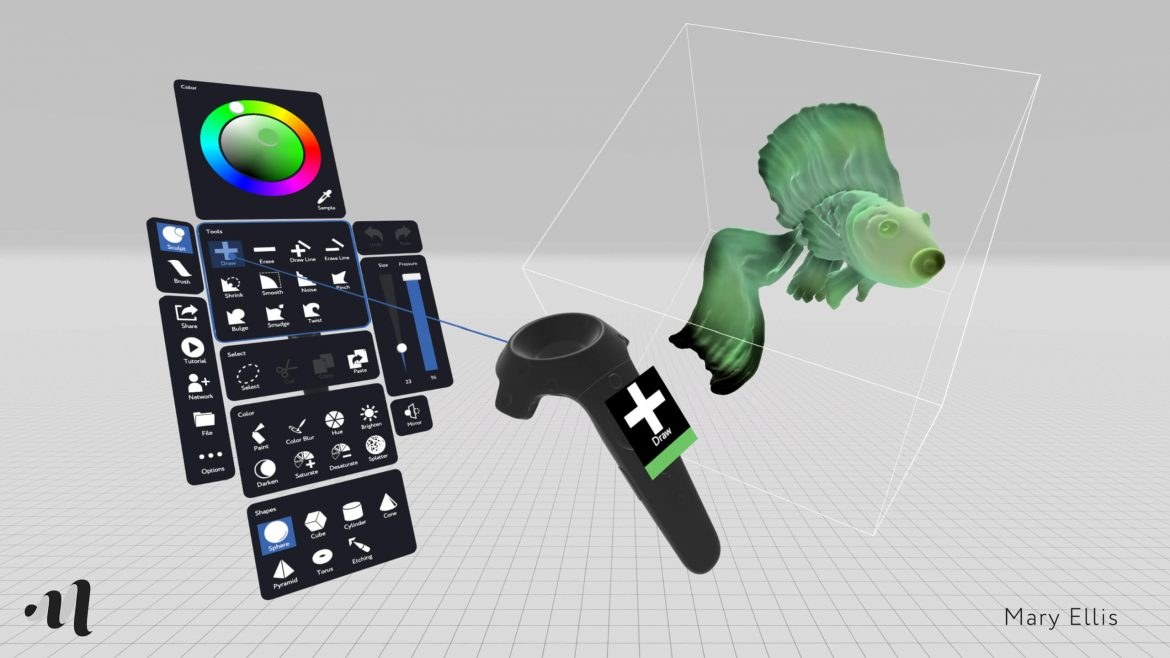
\includegraphics[width=0.5\linewidth]{figures/MasterpieceVR_interface}\\
    (a)&(b)\\
    \end{tabular}
    \caption[MasterpieceVR]{MasterpieceVR.
    	  \textup{(a)} Model of a warrior created in MasterpieceVR by artist Vladimir Ilic.
			  \textup{(b)} Interface of MasterpieceVR (model by Mary Ellis). 
      \label{fig:masterpieceVR}}
\end{figure}

\subsection{Google Blocks}
Google Blocks is available for Oculus and HTC Vive and is Google's software for creating 3D objects in VR. From the programs mentioned in this section, Google Blocks seems the most similar to professional non-VR based modeling software like Blender~\cite{Blender} or Maya~\cite{Maya}. Users can start with several predefined shapes like spheres, cubes or cones and can edit the models on face, edge or vertex level. While this gives the user a lot of artistic freedom and extra modeling possibilities, it also makes its usage a lot less intuitive than the other VR 3D modeling software that is available. Although the user has low-level control, the created meshes are very low-poly compared to the models created with for example Oculus Medium. The user does not have control over the number of polygons, which results in less realistic and smooth models. Again the created models can be exported as .obj file. Figures~\ref{fig:blocks}~(a) and~\ref{fig:blocks}~(b) show a simple model of an anglerfish created in Google Blocks, and the simple Google Blocks interface.

\begin{figure}[!h]
    \centering
    \setlength{\tabcolsep}{0.0130\linewidth}
    \begin{tabular}{@{}cc@{}}
   	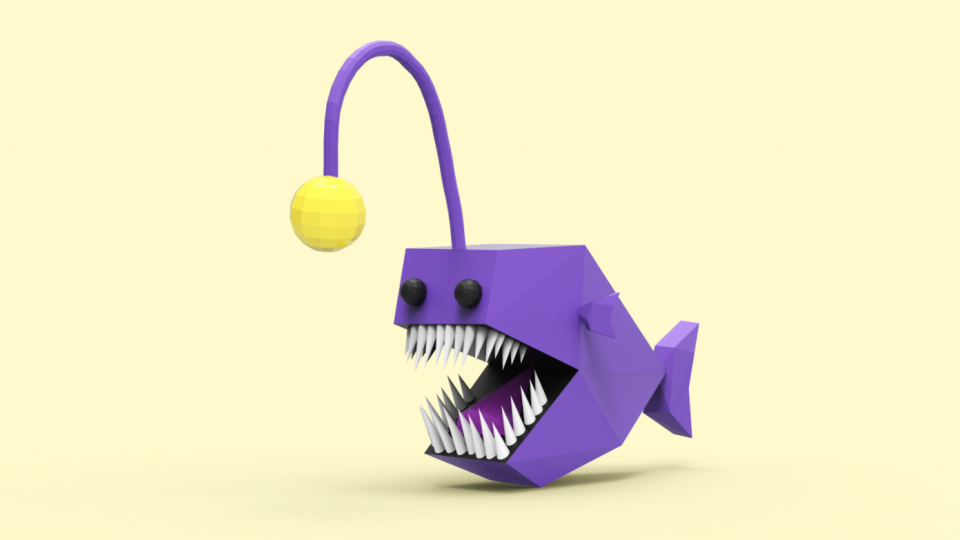
\includegraphics[width=0.487\linewidth]{figures/blocks_anglerfish}&
   	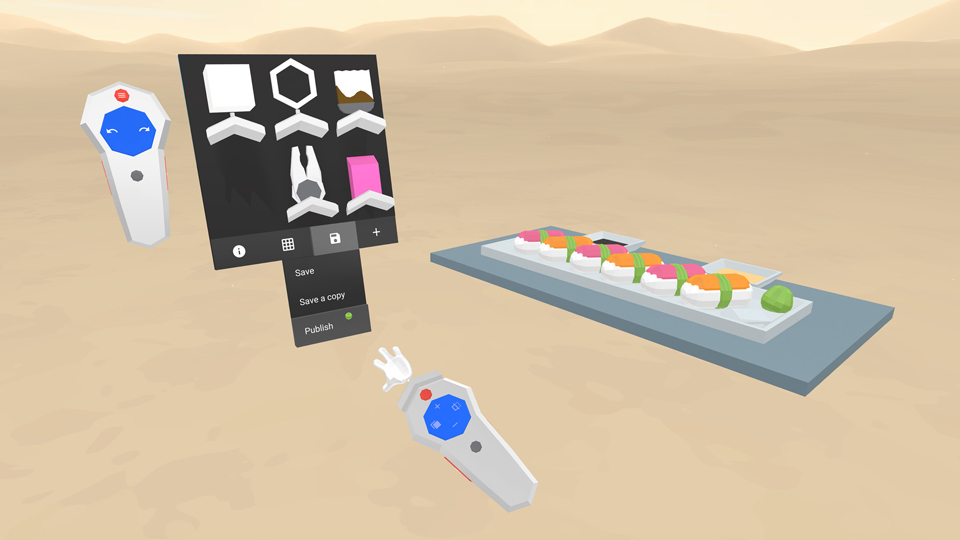
\includegraphics[width=0.487\linewidth]{figures/blocks_interface}\\
    (a)&(b)\\
    \end{tabular}
    \caption[Google Blocks]{Google Blocks.
    	  \textup{(a)} Model of an anglerfish created in Google Blocks.
			  \textup{(b)} Interface of Google Blocks. 
      \label{fig:blocks}}
\end{figure}